Il gruppo di lavoro è composto dagli studenti: Alessandro Cogollo (Cod. Persona: 10571078, Matricola: 938296) e Mario Cela (Cod. Persona: 10685242, Matricola: 937675).

\section{Descrizione globale del progetto}

Il progetto consiste nella realizzazione in linguaggio VHDL di una componente hardware in grado di dialogare con una memoria RAM (descritta nel dettaglio nella sezione successiva), ed elaborare un flusso di bit generato dalla lettura delle parole salvate nella suddetta memoria. Il flusso di bit in output dal convolutore dovrà poi essere salvato in memoria a partire da un dato indirizzo.\\\\
In altre parole, l’hardware da progettare può essere modellizzato con due componenti tra loro strettamente interconnesse: un convolutore di Viterbi, e la struttura di supporto deputata al dialogo con la RAM, alla generazione del bitstream a partire dalle parole di memoria, e al salvataggio delle parole in output.


\section{Note sulla specifica}
Alcune note sulla specifica, fondamentali per la comprensione progettazione dell’hardware, sono riportate in questa sezione.
\\\\
Il modulo inizierà l’elaborazione quando il segnale \codeword{i_start} viene portato a 1, mentre consideriamo terminata l’esecuzione quando \codeword{o_done} viene portato a 1. Ulteriori note sulla relazione tra \codeword{i_start} e \codeword{o_done} sono illustrate nell’apposita sezione relativa all’interfaccia del componente.
\\\\
L’hardware deve quindi essere progettato per poter codificare più flussi in serie; ad ogni nuova elaborazione, il convolutore viene portato nel suo stato iniziale (\textbf{S\_IDLE}), così come vengono reinizializzati gli indirizzi di lettura e scrittura.
\\\\
Assumiamo infine che prima della prima codifica verrà sempre ricevuto dal componente un segnale di \codeword{i_rst}, mentre una seconda elaborazione non dovrà attendere il reset del modulo, ma solo il termine dell’elaborazione.
\\\\
Assumiamo infine che la dimensione massima della sequenza di ingresso sia di 255 byte.


\section{Struttura del convolutore}
Il convolutore rappresenta il cuore del progetto, e il suo funzionamento schematico è riportato in figura qui sotto; il rapporto di codifica utilizzato è 1/2.
\begin{center}
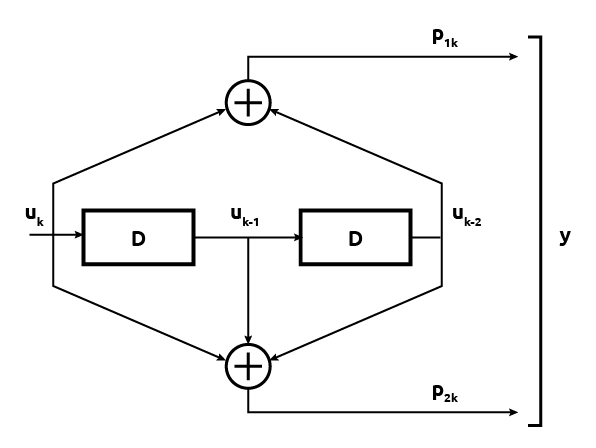
\includegraphics[width=0.7\textwidth]{images/Convolutore.png}
\end{center}

In ingresso al convolutore viene fornito un bitstream che chiameremo \textit{U}, mentre in uscita vengono generati due bitstream \textit{$P_1$} e \textit{$P_2$}. Nello specifico del problema in questione, l’uscita \textit{Y} è composta dall’alternanza, nell’ordine, di \textit{$P_1$} e \textit{$P_2$} (mostrati in figura). Il convolutore è composto da due flip-flop di tipo D; la codifica convoluzionale descritta è considerabile come un caso di codifica con memoria, in quanto l’influenza di un bit in ingresso al tempo \textit{t} si protrae sull’elaborazione di bit in input al tempo \textit{t+1} e \textit{t+2}.
\\\\
La funzione di convoluzione invece è descrivibile come segue:
\begin{center}
    $p_{1k}=u_k+u_{k-2}$
    \\
    $p_{2k}=u_k+u_{k-1}+u_{k-2}$
\end{center}
Lo schema della Finite State Machine (FSM) è riportato nella figura sottostante:

\begin{center}
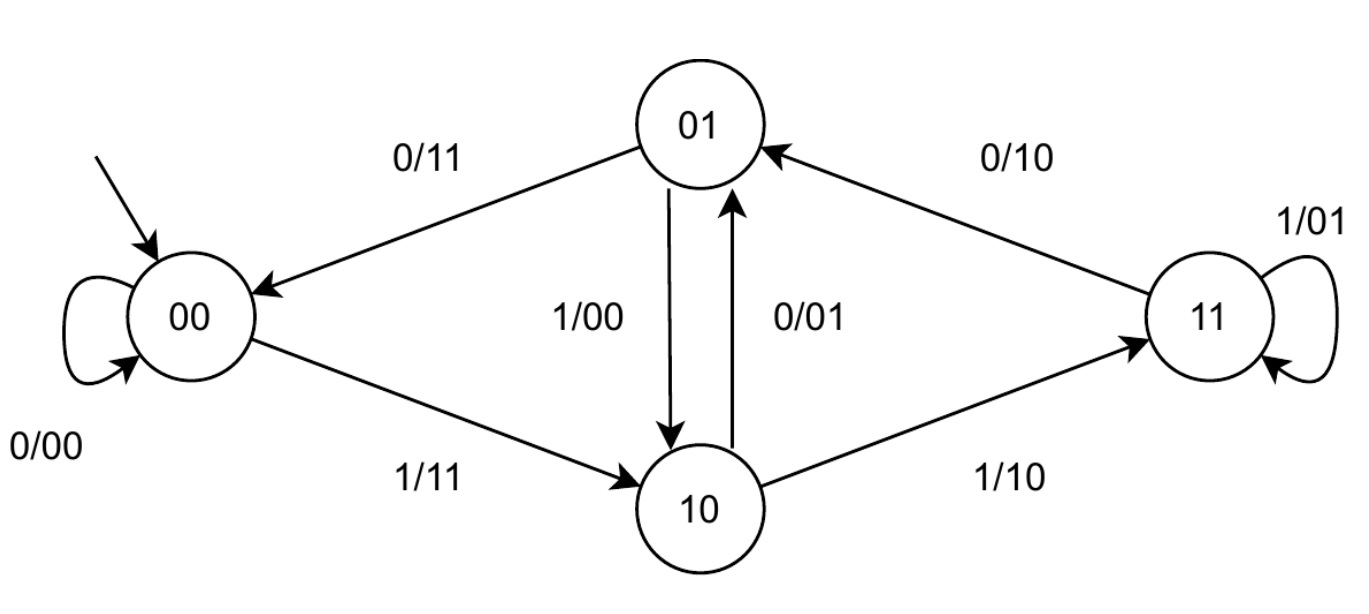
\includegraphics[width=0.89\textwidth]{images/FSM Conv.jpg}
\end{center}

Il codice convoluzionale 1/2 genera 2 bit di output a partire da un singolo bit in input, pertanto è evidente che per ogni parola letta ne verranno salvate due in memoria.


\section{Struttura della RAM}

L’hardware sintetizzato deve interfacciarsi con una memoria RAM di tipo “\textbf{Single-Port Block RAM Write-First Mode}”, in particolare la Random Access Memory è fornita dai template di Xilinx, produttore del software di simulazione e sintesi. Si tratta di una memoria RAM ad accesso \textbf{sequenziale} (single port), che \textbf{prioritizza la scrittura rispetto alla lettura} (write-first mode); entrambe le proprietà vengono specificate in quanto costituiscono casistiche limite che hanno influito sulla progettazione della componente, e nella scrittura dei casi di test, come spiegato nella sezione dedicata.
\\\\
L’interfaccia della memoria è riportata di seguito:\\
\begin{lstlisting}
port(
    clk : in std_logic;
	 we : in std_logic;
	 en : in std_logic;
	 addr : in std_logic_vector(15 downto 0);
	 di : in std_logic_vector(7 downto 0);
	 do : out std_logic_vector(7 downto 0)
);
\end{lstlisting}

L’indirizzamento della parola avviene grazie al segnale \codeword{addr}, che è rappresentato da un array di 16 bit, mentre \codeword{we} ed \codeword{en} costituiscono i segnali di accesso alla memoria, rispettivamente in scrittura ed in lettura; l’accensione del segnale di scrittura richiede l’accensione del segnale di lettura. \codeword{clk} propaga il segnale di clock, mentre \codeword{di} e \codeword{do} rappresentano i segnali in input e output alla memoria.
Da specifica, la memoria può essere idealmente divisa in due parti:

\begin{itemize}
    \item \textbf{Input}: all’indirizzo 0: si trova il numero di parole di input attese, mentre agli indirizzi successivi (fino all’indirizzo 1000 escluso) si trovano le parole che dovranno essere effettivamente elaborate.
    \item \textbf{Output}: dall’indirizzo 1000 alla fine della memoria si riserva lo spazio per la scrittura delle parole elaborate.
\end{itemize}
Un esempio di caricamento della RAM è riportato nella tabella a seguire:
\begin{center}
\begin{tabularx}{\textwidth} {
    | >{\raggedright\arraybackslash}X
    | >{\centering\arraybackslash}X
    | >{\raggedleft\arraybackslash}X | }
    \hline
    Indirizzo           & Parola (binary) & Valore (decimal) \\
    \hline\hline
    0000 0000 0000 0000 & 0000 0011       & 3                \\
    \hline
    0000 0000 0000 0001 & 0111 0000       & 112              \\
    \hline
    0000 0000 0000 0010 & 1010 0100       & 164              \\
    \hline
    0000 0000 0000 0011 & 0010 1101       & 45               \\
    \hline
    [\dots]             & [\dots]         & [\dots]          \\
    \hline
    0000 0011 1110 1000 & 0011 1001       & 57               \\
    \hline
    0000 0011 1110 1001 & 1011 0000       & 176              \\
    \hline
    0000 0011 1110 1010 & 1101 0001       & 209              \\
    \hline
    0000 0011 1110 1011 & 1111 0111       & 247              \\
    \hline
    0000 0011 1110 1100 & 0000 1101       & 13               \\
    \hline
    0000 0011 1110 1101 & 0010 1000       & 40               \\
    \hline
    \hline
\end{tabularx}
\end{center}

\section{Interfaccia del componente}
La specifica del componente richiede che l’interfaccia dell’hardware da implementare sia dotata dei seguenti segnali in ingresso (\codeword{i_}) e uscita (\codeword{o_}).
\\
\begin{lstlisting}
port (
	i_clk : in std_logic;
	i_rst : in std_logic;
	i_start : in std_logic;
	i_data : in std_logic_vector(7 downto 0);
	o_address : out std_logic_vector(15 downto 0);
	o_done : out std_logic;
	o_en : out std_logic;
	o_we : out std_logic;
	o_data : out std_logic_vector (7 downto 0)
);
\end{lstlisting}

In particolare, \codeword{i_clk} è il segnale di clock in ingresso (generato dal TestBench); garantisce un fronte di salita comune tra memoria e componente, fondamentale per eseguire correttamente i test. \codeword{i_rst} è il segnale di reset che inizializza la macchina e la prepara alla ricezione del primo segnale di start. \codeword{i_start} è il segnale di start generato dal TestBench; è richiesto dalla specifica che \codeword{i_start} rimanga alto finché \codeword{o_done} non verrà portato alto, ossia il segnale che notifica la fine dell’elaborazione. Anche il segnale di done deve rimanere alto finché il segnale di start non è riportato a zero. \codeword{i_data} e \codeword{o_data} contengono le parole di memoria in input e output verso la RAM, mentre \codeword{o_address}, \codeword{o_en}, e \codeword{o_we} sono state descritte in precedenza.


\section{Esempio di funzionamento}
Un esempio del funzionamento atteso dal componente è il seguente:

\begin{center}

    \begin{tabularx}{\textwidth}{
        | >{\raggedright\arraybackslash}X
        | >{\raggedright\arraybackslash}X
        | >{\raggedright\arraybackslash}X
        | >{\raggedright\arraybackslash}X | }
        \hline
        Indirizzo           & Parola (binary) & Valore (decimal) & Note                                    \\
        \hline\hline
        0000000000000000 & 0000 0011       & 3                & Sequenza in input       \\
        \hline
        0000000000000001 & 0111 0000       & 112              & $1^{a}$ parola di input  \\
        \hline
        0000000000000010 & 1010 0100       & 164              & $2^{a}$ parola di input \\
        \hline
        0000000000000011 & 0110 1101       & 45               & $3^{a}$ parola di input  \\
        \hline
        \dots             & \dots         & \dots          &                                         \\
        \hline
        \hline
    \end{tabularx}
\end{center}
Le parole in input \textit{W} sono tre: 01110000 10100100 00101101. Seguendo la codifica convoluzionale illustrata precedentemente, ci aspettiamo in output \textit{Z} le seguenti sei parole: 00111001 10110000 11010001 11110111 00001101 00101000, salvate in memoria come segue:
\begin{center}
    \begin{tabularx}{\textwidth}{
        | >{\raggedright\arraybackslash}X
        | >{\raggedright\arraybackslash}X
        | >{\raggedright\arraybackslash}X
        | >{\raggedright\arraybackslash}X | }
        \hline
        Indirizzo           & Parola (binary) & Valore (decimal) & Note                                 \\
        \hline\hline
        \dots              & \dots         & \dots          &                                      \\
        \hline
        0000001111101000 & 0011 1001       & 57               & $1^{a}$ parola di output   \\
        \hline
        0000001111101001 & 1011 0000       & 176              & $2^{a}$ parola di output\\
        \hline
        0000001111101010 & 1101 0001       & 209              & $3^{a}$ parola di output  \\
        \hline
        0000001111101011 & 1111 0111       & 247              & $4^{a}$ parola di output \\
        \hline
        0000001111101100 & 0000 1101       & 13               & $5^{a}$ parola di output \\
        \hline
        0000001111101101 & 0010 1000       & 40               & $6^{a}$ parola di output   \\
        \hline
        \hline
    \end{tabularx}
\end{center}